\normaltrue \difficilefalse \tdifficilefalse
\correctiontrue
%\UPSTIidClasse{11} % 11 sup, 12 spé
%\newcommand{\UPSTIidClasse}{11}

\exer{Triptéor $\star$ \label{CHS:03:B2:16:72}}
%% CCP MP 2007
\setcounter{question}{0}\marginnote{\xpComp{CHS}{03}}%\UPSTIcompetence[2]{B2-16}
\index{Compétence CHS-03}\index{Compétence B2-16}

\index{Tripteor}
\index{Hyperstatisme}

\ifcorrection
\else
\marginnote{\textbf{Pas de corrigé pour cet exercice.}}
\fi

\ifprof
\else
Le triptéor est un centre d'Usinage Grande Vitesse à architecture parallèle, permettent d'envisager un usinage rapide et précis.


\begin{figure}[H]
\centering
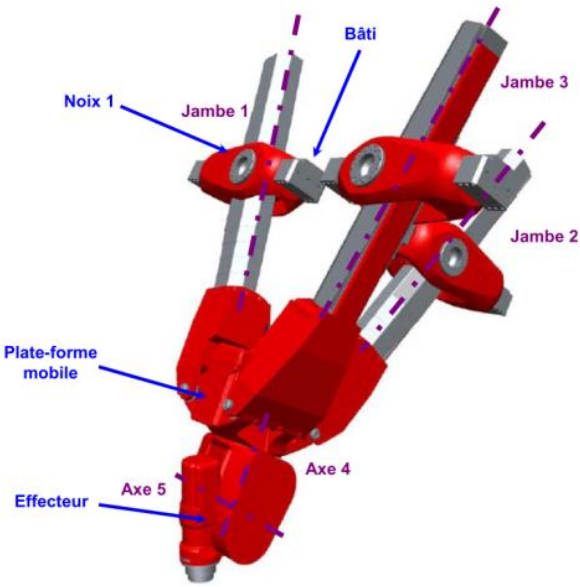
\includegraphics[width=.45\linewidth]{72_01.png}
%\caption{Pince utilisée sur le système ROBOVOLC et schéma cinématique associé \label{fig_23}}
\hfill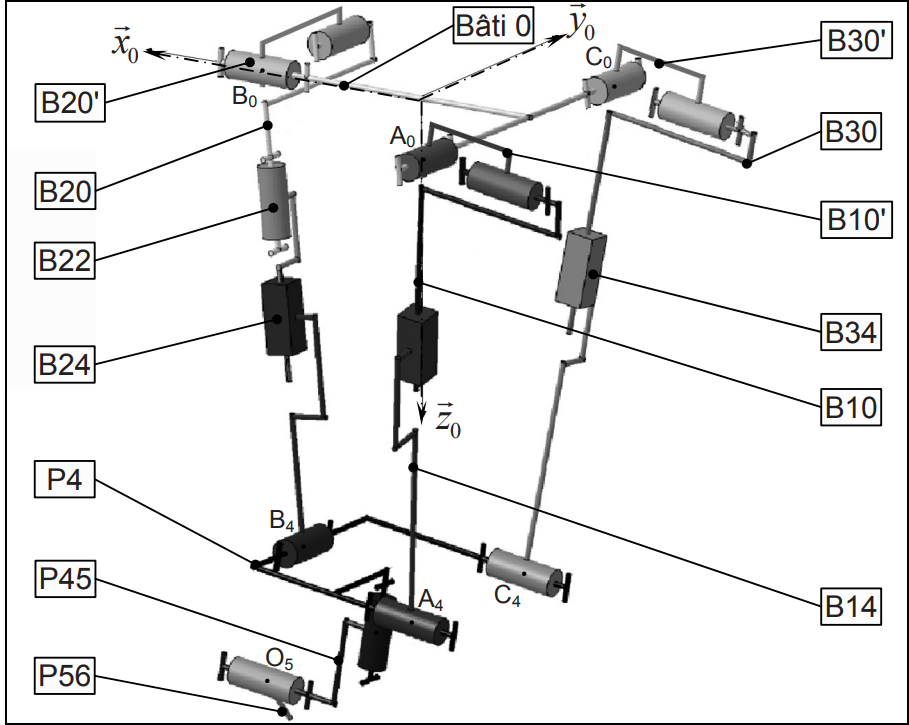
\includegraphics[width=.45\linewidth]{72_02.png}
%\caption{Pince utilisée sur le système ROBOVOLC et schéma cinématique associé \label{fig_23}}
\end{figure}

\fi

\question{Réaliser le graphe de liaisons.}
\ifprof
\begin{center}
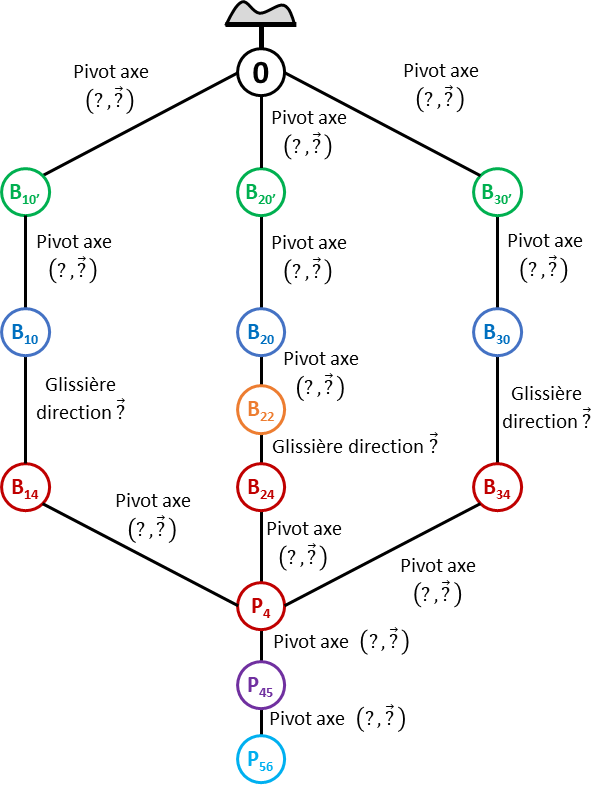
\includegraphics[width=7cm]{72_01_Cor}
\end{center}
\else
\fi

\question{Calculer le degré d'hyperstatisme.}
\ifprof
\begin{itemize}
\item $m=5$ : translations des 3 glissières et rotations des deux dernières pivot;
\item $I_c=15$;
\item $E_c = 12$;
\item $h=m-I_c+E_c = 5 -15 + 12 = 2$.
\end{itemize}
\else
\fi
 

\ifprof
\else
\marginnote[-4cm]{
\begin{solution}
 \begin{enumerate}
\item .
\item $h=2$.
 \end{enumerate}
 \end{solution}
\footnotesize{Corrigé  voir \ref{CHS:03:B2:16:72}.}}%
\fi